	\documentclass[10pt,oneside]{CBFT_book}
	% Algunos paquetes
	\usepackage{amssymb}
	\usepackage{amsmath}
	\usepackage{graphicx}
% 	\usepackage{libertine}
% 	\usepackage[bold-style=TeX]{unicode-math}
	\usepackage{lipsum}

	\usepackage{natbib}
	\setcitestyle{square}

	\usepackage{polyglossia}
	\setdefaultlanguage{spanish}
	



	\usepackage{CBFT.estilo} % Cargo la hoja de estilo

	% Tipografías
	% \setromanfont[Mapping=tex-text]{Linux Libertine O}
	% \setsansfont[Mapping=tex-text]{DejaVu Sans}
	% \setmonofont[Mapping=tex-text]{DejaVu Sans Mono}

	%===================================================================
	%	DOCUMENTO PROPIAMENTE DICHO
	%===================================================================

\begin{document}

% =================================================================================================
\chapter{Elementos de la teoría de fenómenos críticos}
% =================================================================================================


% =================================================================================================
\section{Ising 1}
% =================================================================================================

El modelo de Ising intenta explicar el ferromagnetismo. El estado espontáneo es spines desordenados
(no hay magnetización). Considero solo interacciones entre primeros vecinos.
Si cambio todo un bloque a lo sumo solo hay un cambio en la frontera, porque las interacciones son
entre primeros vecinos.

El proceso de ``generar paredes'' minimiza el $A$ y desordena y aumenta la $S$ de manera que el sistema
evoluciona así. Este es el modelo de Ising en 1D. En 2D se complica sobremanera.
La cantidad $\chi(b,i)$ camina sobre todos los dominios en una sola configuración.
Hay regiones donde se da la magnetización espontánea en Ising 2D.


\begin{itemize}
 \item Modelo sencillo de sistema interactuante
 \item Magnetización espontánea 1D y 2D:
 \subitem En 1D no hay magnetización espontánea
 \subitem En 2D hay magnetización espontánea
\end{itemize}

Fase es una porción de materia física y químicamente homogénea (asociada a la densidad atómica o molecular
uniforme) que no puede separarse por medios mecánicos.

Una fase puede ser una única sustancia o una mezcla.

El concepto de fase está también relacionado con el pasaje de la materia de una a otra fase.

\notamargen{corregir}

Estados de agregación (en función de la proximidad de sus componentes). Agua y aceite (líquido) es un sistema de dos 
fases.

La materia puede encontrarse en gran variedad de fases; las más conocidas están relacionadas con los estados de 
agregación. Pero dentro del estado sólido tenemos fases dependiendo de cómo sea la estructura interna.

Tenemos también sistemas que manifiestan fases ordenadas y desordenadas; aleaciones de sólidos, superconductividad.

Transición de fase: cuando una propiedad del sistema cambia discontinuamente frente a la variación de un parámetro 
intensivo ($T, p$ campo magnético).

\[
	\text{ interacciones entre partículas } \; \longrightarrow \; \text{ CORRELACIÓN A GRAN ESCALA }  
\]

Las transiciones de fase emergen de la interacción. Uno de los modelos más sencillos fuera del gas ideal es el modelo de
Ising (red con interacción entre primeros vecinos)
\[
	\boxed{ E_\nu = -H \sum_{i=1}^N (\mu S_i) - J \sum_{\braket{i,j}} S_i \cdot S_j }
	\label{energia_ising}
\]
\notamargen{Ising es energía dada por \eqref{energia_ising} e interacción a primeros vecinos.}

dibujo 


donde $\nu$ es una dada configuración de la red (valores $S_i$ con $i=1,2,...,N$)
\[
	S_i = \pm 1 \qquad \rightarrow \qquad \pm \mu S_i \text{ Momento magnético del spin i-ésimo }
\]
donde $\mu>0$, $J$ es constante de acoplamiento y $\sum_{<i,j>}$ se extiende sobre los pares de vecinos (primeros).

Con $J>0$ es favorable que todos los spines se hallen alineados. Entonces esto llevará a la magnetización espontánea: 
fenómeno de cooperación; la mayoría de los spines se orienta en una dirección y dan un valor de magnetización 
$\braket{M} \neq 0$
\[
	M_\nu = \sum_{i=1}^N \mu \cdot S_i^\nu
	\text{ (Magnetización) }
\]
\notamargen{$J>0$ ferromagnetismo y $J<0$ paramagnetismo}

Si los spines están orientados al azar, entonces habrá igual cantidad de $+1$ que de $-1$ y entonces
\[
	M \approx 0
\]

Si $H=0$ entonces $M$ es la magnetización espontánea.
\notamargen{$M$ se define como un momento dipolar magnético por unidad de volumen.}

Habrá magnetización con $T$ baja (o $J$ alto) y hasta una $T_\text{curie}$
\[
	Q_N(H,T) = \sum_{s_1=-1}^{+1} \; \sum_{s_2=-1}^{+1} \; ... \sum_{s_N=-1}^{+1} \;
	\euler^{ +\beta H \mu \sum_i^N S_i + \beta J \sum_{\braket{i,j}} S_i \cdot S_j }
\]
donde las sumatorias toman para cada $i$ los valores $S_i = +1, -1$
\[
	A = -kT\log Q \qquad \braket{E} = -\dpar{}{\beta}\log Q = kT^2 \dpar{}{T} \log Q
\]

Me interesa definir densidades de $ N_+, N_{++} $

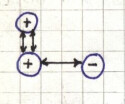
\includegraphics[scale=0.4]{images/1606337009.jpg}

y consideraremos un efecto promedio
\[
	\frac{ N_{++} }{ N y/2 } = \Frac{ N_{+} }{ N }^2
\]
que es una aproximación de campo medio, definiendo un $L$ tengo muchos $\{ S_i \}$.
Al eliminar $\sigma$ perdemos la estructura fina de la red y hacemos estadística allí.

El campo magnético rompe la degeneración pues dessimetriza. Luego con $ H \to 0 $ y me quedo
con la curva que resultó no simétrica (el $A$ deja de ser simétrico).

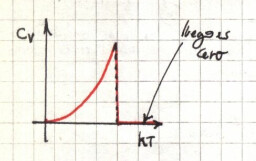
\includegraphics[scale=0.4]{images/1606337012.jpg}

Esto es la aproximación de Bragg-Williams, que ha descartado las correlaciones; entonces
hemos contado nodos.
La aproximación de Bethe-Peierls tomo como unidades fundamentales

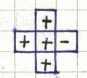
\includegraphics[scale=0.4]{images/1606337015.jpg}

$P(+,n)$ es la probabilidad condicional de tener un $+$ en el nodo central mientras que
$P(-,n)$ es la de tener un $-$ en el nodo central.
Otra apromicaicón
\[
	\frac{ N_{++} }{ N y/2 } = \frac{1}{2}( \sigma + 1 )
\]

El efecto del resto del sistema es una $ z = \euler^{\beta \mu} $ asociado a la influencia
del resto del sistema.

\[
	\sum_{n=0}^\gamma \: P(+,n)
\]
y sumo sobre todos los posibles vecinos hasta $\gamma$.

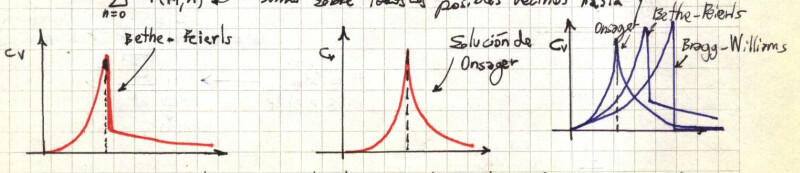
\includegraphics[scale=0.4]{images/1606337019.jpg}

Las fluctuaciones de la energía del sistema nos darán el calor específico $C_V$ (como en el $Z_{GC}$).
Se puede pensar como una transición del orden al desorden. En 2D tenemos magnetización espontánea.

\begin{ejemplo}{(Ejercicio 5.1 Chandler)}
\[
	E_0 = -J \sum_{\braket{i,j}} S_i \cdot S_j = -J  \sum_i^N \sum_j^\gamma \frac{S_i S_j}{2}
\]
para cada $i$ sumo en sus $\gamma$ vecinos el $j$ (sobre 2 para no contar dos veces).
\[
	E_0 = -J \sum_i^N \frac{S_i\gamma}{2} = -J N\frac{\gamma}{2} = -JND
\]
donde $D$ es la dimensionalidad.
\end{ejemplo}


Como es
\[
	E_\nu =  -H \sum_{i=1}^N \mu \cdot S_i - J \sum_{\braket{i,j}} S_i \cdot S_j \qquad
	\text{ y } \qquad \braket{M} = \braket{ \sum_i^N \mu \cdot S_i }
\]
entonces
\[
	\braket{M} = \braket{ \sum_i^N \mu \cdot S_i } = 
	\frac{ \sum_{s_1} \; \sum_{s_2} \; ... \sum_{s_N} \;
	\euler^{ \beta H \mu \sum_i^N S_i + \beta J \sum_{\braket{i,j}} S_i \cdot S_j } }{Q_N}
\]
\[
	\braket{M} = \frac{ \sum_{s_1} \; \sum_{s_2} \; ... \sum_{s_N} \;
	\dpar{}{\beta H} \left[ \euler^{ \beta H \mu \sum_i^N S_i + \beta J \sum_{\braket{i,j}} S_i \cdot S_j } 
	\right]}{Q_N} = \frac{\dpar{}{\beta H}(Q_N)}{Q_N}
\]
\[
	\braket{M} = \dpar{}{\beta H}\left( \log Q_N \right) = \dpar{}{\beta H}\left( -\beta A \right) =
	\dpar{}{H}\left( A \right)
\]

\subsection{No hay magnetización espontánea en 1D}

\notamargen{Error en Huang (14.6); es $-\dpar{}{H}(A_I)$}

DIBUJO 

Con $H=0$ invierto spines detrás de una pared.
\[
	E_0 = -J(N-1) \qquad E_f = -J[(N-1)-2p]
\]
\notamargen{$p$ es el número de paredes}

Varían los términos asociados a la pared
\[
	\Delta E = E_f - E_0 = 2Jp > 0
\]
con $p=1$ es $\Delta E = 2J$ y con $p=2$ es $\Delta E = 4J$ (es 2 por pared puesto que desaparece un $+$ y aparece
en su lugar un $-$).

La variación de $S$ está asociada con el número de formas de ubicar la pared
\[
	S = l \log (N-1)
\]
y es la $S$ del estado con una pared, el desordenado.
\[
	\Delta S = k \log(N-1)	\qquad (S_0 \equiv 0)
\]
que define al estado sin pared como de entropía $S_0=0$
\[
	A = U - TS \quad \rightarrow \quad \delta A = \delta U - T \delta S
\]
\[
	\delta J - kT \log(N-1)
\]
\notamargen{Para $p$ paredes es 
$\Delta A = 2Jp - kT \log [(N-1)(N-2)...(N-p)]$}

Con $T > 0$ tenemos que si desordeno (agrego paredes) sube $U$ y sube $S$.
En general, como 
\[
	\frac{\delta A}{kT} = \frac{2J}{kT} - \log(N-1)
\]
vemos que para $N\to\infty$ $\delta A < 0$ a menos de que $J/kT$ sea muy grande.

\notamargen{$S$ domina la minimización de $A$.}

En un sistema macroscópico 1D el desorden baja la $A$, entonces el equilibrio tiende
al desorden (no al orden).

Es decir, un sistema 1D de spines a $ T \neq 0 $ espontáneamente irá hacia $ A $
mínimas (mayor aleatoriedad), no se tiende a alcanzar estados ordenados.

\subsection{Magnetización espontánea en 2D}

La magnetización media por spín es
\[
	\mathcal{M} = \frac{1}{2} \Frac{N_+ - N_-}{N}
\]
Con $N\to\infty$ claramente será 0 a no ser que exista una preferencia por cierta dirección $+$ o $-$.

Queremos calcular todas las configuraciones posibles de un arreglo 2D de spines.
Para ello sistematizamos una dada construcción en dominios $\Box$ que engloban spines ($-$) y están
limitados por paredes.

DIBUJO ising


Los spines $+$ son una condición de contorno que con $N\to\infty$ es una perturbación que rompe la
simetría. También sirven para cerrar los dominios.

Cada dominio tiene una longitud $b$ medido en paredes $|$ y una dirección de recorrido de forma que 
los spines $-$ están siempre a la izquierda de la pared.
El tamaño de la red es $\sqrt{N} \times \sqrt{N} = N$. El área se mide en términos del dominio 
mínimo ``$\Box$''
\[
	\text{ dominio } = (b,i)
\]
donde $b$ es el número de paredes e $i$ una etiqueta.

A un mismo número de paredes según forma y localización tendrá varios dominios.

Una dada configuración del sistema tendrá ciertos dominios $(b,i)$

\begin{center}
\begin{tabular}{llll}
 & $b$ (paredes) & Areas (spines) & $b^2/16$ \\
\hline
 & 4 & 1 & 1\\
 & 6 & 2 & 2.25\\
 & 8 & 3,4 & 4
\end{tabular}
\end{center}

Si cada spin ocupa un área de 1, en términos de paredes el área que engloba un dominio de $b$ paredes
es 
\[
	\text{ Área dominio } \neq \frac{b^2}{16} \qquad \rightarrow \qquad S([b,i]) = \text{ Área dominio}
\]
\notamargen{Tengo una figura de longitud $b$ y si la quiero llevar a un cuadrado con suerte el lado
será $b/4$ de modo que su área es $b^2/16$}

Definimos ahora 
\[
	\chi([b,i]) = \begin{cases}
	              1 \qquad \text{ Si (b,i) ocurre en una dada configuración } \\
	              0 \qquad \text{ En caso contrario}
	             \end{cases}
\]
y $m(b)$ número de dominios de $b$ paredes.

Luego;
\[
	\boxed{ N_- = \sum_b \sum_i^{m(b)} \chi([b,i]) S([b,i]) } \quad [1]
\]
en el caso dibujado sería
\[
	N_- = 1 \cdot S(6,i) + 1 \cdot S(8,i') + 1 \cdot S(26,i'') \qquad 
	N_- = 1 \cdot  2 + 1 \cdot  4 + 1 \cdot 12 = 18
\]

Por la [1] se puede acotar, empezando por $m(b)$. Para ver el número de dominios de longitud $b$ piénsese que 
para la primera pared tengo $N$ posibilidades; para las siguientes $b-1$ tengo tres opciones pues no puedo volver,
y entonces 
\[
	m(b) \leq N 3^{b-1}
\]

Nótese que estamos considerando paredes abiertas y cerradas.

Luego,
\[
	\braket{N_-} \leq \sum_b \sum_i^{N3^{b-1}} \chi([b,i]) \underbrace{S([b,i])}_{\leq b^2/16}
\]
\[
	N_- \leq \sum_b \frac{b^2}{16} \sum_i^{N3^{b-1}} \chi([b,i])
\]
\[
	\braket{N_-} \leq \sum_b \frac{b^2}{16} \sum_i^{N3^{b-1}} \braket{\chi([b,i])}
\]

Pero
\[
	\braket{\chi([b,i])} = \frac{ \sum_{\{Si\}}' \euler^{-\beta E_{\{Si\}}} }
	{ \sum_{\{Si\}} \euler^{-\beta E_{\{Si\}}} }
\]
donde la sumatoria es en aquellas configuraciones que contienen al dominio $(b,i)$.

\notamargen{num: de todas las configuraciones posibles aquellas en las cuales se da el dominio $(b,i)$.
den: todas las configuraciones posibles.}

Removemos términos del denominador para acotar: pensamos que si en una dada configuración $C$ con $\{b,i\}$ revertimos 
en el dominio $\{b,i\}$ los spines llegamos a una configuración $\tilde{C}$
\[
	E_C - E_{\tilde{C}} = 2 \varepsilon b
\]

Al revertir los spines de un dominio pasamos a una configuración más ordenadas y por ende de menor energía
 
 DIBUJO
 
\[
	\frac{ \sum_{\{Si\}}' \euler^{-\beta E_{\{Si\}}} }{ \sum_{\{Si\}} \euler^{-\beta E_{\{Si\}}} }
	\leq 
	\frac{ \sum_{\{C\}} \euler^{-\beta E_C} }{ \sum_{\{C'\}} \euler^{-\beta E_{\tilde{C}}} } =
	\frac{ \sum_{\{C\}} \euler^{-\beta E_C} }{ \sum_{\{C\}} \euler^{-\beta E_{\tilde{C}}} 
	\euler^{2\beta\varepsilon b} } = \euler^{-2\beta \varepsilon b}
\] 
\[
	\braket{N_-} \leq \sum_b \frac{b^2}{16} \euler^{-2\beta \varepsilon b} N 3^{b-1} =
	\frac{N}{48} \sum_b b^2 [ 3 \euler^{-2\beta \varepsilon } ]^b
\]
\[
	\braket{N_-} \leq \frac{N}{48} \sum_{b=4,6,8,...} b^2 x^2,
\]
con $ x \equiv 3 \euler^{-2\beta \varepsilon } $

\[
	\braket{N_-} \leq \frac{N}{48} (16x^4 + 36x^6 + 64x^8 + ...) 
\]
Sea $b=2n$, entonces
\[
	\braket{N_-} \leq \frac{N}{48} \sum_{n=2,3,4,...} 4 n^2 (x^2)^n,
\]
con $x^2 = 9 \euler^{-4\beta\varepsilon} $
\[
	\braket{N_-} \leq \frac{N}{12} \sum_{n=2}^\infty n^2 r^n,
\]
con $r=9 \euler^{-4\beta\varepsilon}$
\[
	\braket{N_-} \leq \frac{N}{3} \frac{r^2}{(1-r)^3} \left[ 1 - \frac{3}{4}r + \frac{1}{4}r^2 \right]
\]
y esta cantidad para algún $\beta$ grande pero finito es menor a $N/2$.


% =================================================================================================
\section{Ising 2}
% =================================================================================================

La energía se podía escribir como
\[
	E_\nu = - H \sum_i^N (\mu s_i) - J \sum_{\braket{i,j}} s_i \cdot s_j 
\]

El grado de un nodo es $\gamma$ que depende de la red y de la dimensión,
\begin{center}
\begin{tabular}{lll}
2D & cuadrada & $\gamma=4$ \\
3D & SC & $\gamma=6$ \\
3D & BCC & $\gamma=8$
\end{tabular}
\end{center}

\notamargen{$\gamma$ es el número de vecinos. De cada nodo salen $\gamma$ líneas.}

\[ 
	\sum_{\braket{i,j}} = \frac{\gamma N}{2} = \text{ nro total de líneas } 
\]

dibujos

Tomando un nodo y trazando líneas a sus $\gamma$ vecinos tengo $ \gamma N/2 $ líneas dibujadas
(se divide en 2 por el doble conteo).

Tomando cada $\oplus$ trazo líneas a sus vecinos y defino
\[ 
	N_+ = \text{ nro de spines $\uparrow$} \qquad N_- = \text{ nro de spines $\downarrow$}
\]
\[ 
	N_{++} = \text{ nro de pares $\uparrow\uparrow$} \qquad 
	N_{--} = \text{ nro de pares $\downarrow\downarrow$}
\]
\[ 
	N_{+-} = \text{ nro de pares $\uparrow\downarrow$ o ($\downarrow\uparrow$)}
\]
\begin{itemize}
 \item 1) $ \gamma N_+ = 2N_{++} + N_{+-} $
 \item 2) $ \gamma N_- = 2N_{--} + N_{+-} $
 \item 3) $ N_+ + N_- = N $
\end{itemize}

\[
	\gamma N = 2N_{++} + 2N_{--} + 2N_{+-}
\]
\[
	\gamma N_+ + \gamma N_- = (2N_{++} + N_{+-}) + (2N_{--} + N_{+-})
\]
\[
	\frac{\gamma N}{2} = N_{++} + N_{--} + N_{+-} 
\]

Podemos poner todo en términos de $N_{++}, N_+, N$ y entonces
\[
	N_{+-} = \gamma N_+ - 2N_{++} \qquad N_- = N - N_+
\]
\[
	N_{--} = \frac{\gamma}{2}(N-N_+) - \frac{1}{2}(\gamma N_+ - 2N_{++}) =
	\frac{\gamma}{2} N - \gamma N_+ + N_{++}
\]
\begin{multline*}
	\sum_{\braket{i,j}} s_i \cdot s_j = N_{++} + N_{--} - N_{+-} =
	N_{++} + \frac{\gamma}{2}N - \gamma N_+ + N_{++} - \gamma N_+ + 2N_{++}= \\
	4N_{++} - 2\gamma N_+ + \frac{\gamma}{2}N 
\end{multline*}
\[
	s_i = N_+ - N_- = N_+ - (N-N_+) = 2N_+ - N
\]

La energía se puede escribir en función de estas variables
\[
	E_I = - H\mu (2N_+ - N) - J(4N_{++} - 2\gamma N_+ + \frac{\gamma}{2}N)
\]
\[
	E_I = -4JN_{++} - 2(H\mu - \gamma J)N_+ - \left( \frac{\gamma J}{2}- H\mu \right)N
\]

\notamargen{La energía depende de las cantidades $N,N_+,N_{++}$ y no del detalle de la distribución
de los mismos.}

La función canónica será
\[
	Q_I = \sum_{E_I} \euler^{-\beta E_I} = \euler^{\beta(J\gamma/2 - H\mu)N } \sum_{N_+=0}^N
	\left( \euler^{2\beta( \mu H - J\gamma )N_+ } \sum_{N_{++}}' \euler^{4\beta J N_{++}}
	\: g(N_+,N_{++})\right)
\]
donde $g(N_+,N_{++})$ es el número de configuraciones de $N_{++}$ y $N_{+}$ y la sumatoria primada se hace 
sobre los valores de $N_{++}$ consistentes con que hay $N_{+}$ spines up.

Esta expresión no ha sido resuelta salvo en 2D.

\subsection{Aproximación de Bragg-Williams}

\[
	\frac{N_+}{N} = \text{ (promedio) $\leftarrow$ correlaciones de largo rango } 
\]
\[
	\frac{N_{++}}{\gamma/2 N} = \text{  $\leftarrow$ correlaciones de corto rango } 
\]
y entonces $N_{+}/N$ está asociado a una visión global del sistema (un cuerpo), 
mientras que $N_{++}/(\gamma/2 N)$ lo está a una visión local del sistema (dos cuerpos).

Si un dado spin es $\oplus$ entonces tiene en promedio $N_{++}/(\gamma/2 N)$ vecinos del tipo $\oplus$.

Definimos unos parámetros de orden $L$ y $\sigma$
\[
	\frac{N_+}{N} = \frac{1}{2}(L+1) \qquad (\text{ todo } \downarrow) -1 \leq L \leq 1 (\text{ todo } \uparrow)
\]
\[
	\frac{N_{++}}{\gamma/2 N} = \frac{1}{2}(\sigma + 1) \qquad -1 \leq \sigma \leq 1
\]
\notamargen{Estamos viendo todo del lado de los spines $\oplus$.}
pero 
\[
	\sum_i s_i = 2N_+ - N = (L+1)N - N = NL,
\]
\[
	\braket{M} = \braket{ \sum_i^N \mu s_i } = \mu \braket{ \sum_i^N s_i } = \mu N \braket{L} 
\]
\[
	\frac{\braket{M}}{\mu N} \equiv \mathcal{M} = \braket{L}
\]
que es la magnetización por partícula (adimensional).
\[
	\sum_{\braket{i,j}} = \frac{1}{2} N \gamma (2\sigma - 2L + 1) 
\]

La energía es 
\[
	E = - H \mu \sum_i^N s_i - J \sum_{\braket{i,j}} =
	-H\mu NL - \frac{J}{2} N \gamma (2\sigma - 2L + 1) 
\]
y por partícula,
\[
	\epsilon \equiv \frac{E}{N} = -H\mu L - \frac{J}{2} \gamma (2\sigma - 2L + 1) 
\]

Hasta aquí el planteo es exacto; Bragg-Williams hace la aproximación
\notamargen{Significa que no hay correlaciones de orden corto salvo las que surgen
del orden largo. Me quedo sólo con el parámetro $L$.}
\[
	\frac{N_{++}}{\gamma/2 N}= \Frac{N_+}{N}^2
\]
\[
	\frac{1}{2}(\sigma + 1) \approx \frac{1}{2^2} (L+1)^2 \quad \rightarrow \quad 
	\sigma \approx \frac{L^2 + 2L + 1}{2}
\]
\[ 
	\boxed{ E = -\mu H N L - \frac{JN\gamma }{2}L^2 },
\]
que es la $E$ en Bragg-Williams.
\[
	Q(H,T) = \sum_{\{ s_i\}} \euler^{-\beta N(- H\mu L - JL^2 \gamma / 2) }
\]
donde $\{ s_i\}$ es la configuración de los N spines.

La suma se extiende sobre todos los conjuntos $\{ s_i\}$, pero el sumando sólo depende de $L$.
Queremos saber cuántos conjuntos $\{ s_i\}$ tienen el mismo $L$,
\[
	\frac{N!}{N_+!(N-N_+)!}
\]
que es el número de maneras de tomar $N_+$ de $N$ indistinguibilizando dentro de $N_+$ y de $N_-\equiv
N-N_+$
\[
	Q(H,T) = \sum_{L=-1}^{L=1} \frac{N!}{N_+!(N-N_+)!}
	\euler^{\beta N( H\mu L + JL^2 \gamma / 2) }
\]

La suma es ahora en todos los $L$ posibles. Con $N\to\infty$ el logaritmo de $Q$ es dominado por el término
(con $\bar{L}$) que maximiza el sumando.
\notamargen{La clave es el término que maximiza el sumando en valor absoluto. Será máximo o mínimo. }
\[
	\log (Q(H,T)) = \log \left( \sum_L \frac{N!}{N_+!(N-N_+)!} \euler^{\beta N f(L)} \right)
\]
si pensamos que la suma está dominada por un término,
\[
	\log (Q(H,T)) \approx \log \left( \frac{N!}{ N/2(\bar{L}+1)!N/2(1-\bar{L})!} 
	\euler^{\beta N f(\bar{L})} \right)
\]
\[
	\log (Q(H,T)) \approx \log N! - \log N/2(\bar{L}+1)!N/2(1-\bar{L})! + 
	\beta N ( H\mu \bar{L} + J\bar{L}^2 \gamma/2 ) 
\]
y usando Stirling,
\[
	\log Q = \beta N H \mu \bar{L} + \beta \frac{NJ}{2} \gamma \bar{L}^2 -
	\frac{N}{2} \log \Frac{1-\bar{L}^2}{4} - \frac{N\bar{L}}{2} \log \Frac{1+\bar{L}}{1-\bar{L}}
	\qquad [1]
\]
pero no sabemos quién es $\bar{L}$. Y si hacemos
\[
	\dpar{}{\bar{L}}( \log Q[H,T] ) = 0
\]
llegamos a que debe valer [2]
\[
	\log \frac{1+\bar{L}}{1-\bar{L}} = 2\beta H\mu + 2\beta \gamma \bar{L} J
\]
y por ello el valor de $\bar{L}$ sale de
\[
	\bar{L} = \tanh( \beta H \mu + \beta \gamma J \bar{L} )
\]

Con $H=0$ es 
\[
	\boxed{ \bar{L} = \tanh( \beta \gamma J \bar{L} ) } \qquad \text{ condición para $\bar{L}$ }
\]

DIBUJO 

busco igualar $f=\tanh(\beta\gamma J\bar{L})$ con $f=\bar{L}$.

Entonces, si
\[
	T_c \equiv \frac{\gamma J}{k} > T \qquad \rightarrow \quad \bar{L} = 0, L_0, -L_0 \; 
	\text{ son soluciones } 
\]
\[
	T_c \equiv \frac{\gamma J}{k} \geq T \qquad \rightarrow \quad \bar{L} = 0 \; 
	\text{ es solución } 
\]
siendo $T_c$ la temperatura de Curie.
\notamargen{El $L$ máximo, el $\bar{L}$, es el que domina en $\log Q$.
Asimismo, como $A = -kT\log Q$, el valor que maximiza $\log Q$ también minimiza $A$.}
Usando (2) en (1) podemos escribir 
\[
	- \beta A = \log Q(H,T) \approx - \beta \frac{\gamma J N}{2} \bar{L}^2 
	- \frac{N}{2} \log \Frac{1-\bar{L}^2}{4}
\]
\[
	\log Q(H,T) \approx - \Frac{T_c}{T}\frac{N}{2}\bar{L}^2 - \frac{N}{2} \log \Frac{1-\bar{L}^2}{4}
	\; [3]
\]
pero (3) vale para el $\bar{L}$ que maximiza $\log Q$. Vemos que es independiente de $H$.
Es más, (3) graficado en función de $\bar{L}$ no me dice nada. Lo que es valioso es (1).
Desde allí,
\[
	A \approx -NH\mu \bar{L} - kT_C \frac{N}{2}\bar{L}^2  + kT\frac{N}{2} \log \Frac{1-\bar{L}^2}{4}
	+ kT \frac{N}{2} L \log \Frac{1+\bar{L}}{1-\bar{L}}
\]

Considerando $H=0$ resulta
\[
	\frac{\beta A}{N/2} \approx -\frac{T_c}{T} \bar{L}^2 + \log \Frac{1-\bar{L}^2}{4}
	+ \bar{L} \log \Frac{1+\bar{L}}{1-\bar{L}}
\]
y si 
\[
	-\frac{2H\mu}{kT}\bar{L},
\]
siendo chico el factor,

DIBUJOS

\[
	A \approx k T_c \frac{N}{2} \bar{L}^2 + k T N \log \Frac{1-\bar{L}^2}{4}
\]

El efecto del $H\neq 0$ es entonces romper la degeneración. Por otro lado $\bar{L}$ es el valor de
magnetización por partícula. Entonces podemos graficar $A(\mu)$

DIBUJO

Las otras funciones termodinámicas resultan (con $H=0$)
\[
	\frac{M}{\mu N} = \begin{cases}
	                   0 \qquad T > T_c \\
	                   L_0 \qquad T< T_c
	                  \end{cases}
\]
\[
	\frac{A}{N} = \begin{cases}
	                   0 \qquad T > T_c \\
	                   \frac{\gamma J}{2}\bar{L_0}^2 + \frac{kT}{2} \log \Frac{1-\bar{L_0}^2}{4}
	                   \qquad T< T_c
	                  \end{cases}
\]
\[
	\frac{U}{N} = \begin{cases}
	                   0 \qquad T > T_c \\
	                   -\frac{\gamma J}{2}\bar{L_0}^2 \qquad T< T_c
	                  \end{cases}
\]
\[
	\frac{C}{N} = \dpar{}{T}\Frac{U}{N} = \dpar{}{T}\left(-\frac{\gamma J}{2}\bar{L_0}^2 \right)
	= - \gamma J L_0 \dtot{L_0}{T}
\]
donde $L_0$ debe computarse numéricamente pero podemos aproximar en dos límites $T\approx 0$ y $T\approx T_c$

\[
	L_0 = \tanh\Frac{T_c L_0}{T} = \frac{(1-\euler^{-2x})}{1+\euler^{-2x}}
	\approx (1-\euler^{-2x})^2
\]
siendo $x\equiv T_cL_0/T$ y amasando tenemos
\[
	\begin{cases}
	L_0 \approx 1 - 2\euler^{-T_cL_0/T} \quad \text{ si } T_c/T \gg 1 \\
	L_0 \approx 3^{1/2}\left( 1 - \frac{T}{T_c} \right)^{1/2} \quad \text{ si } T_c \approx T 
	\end{cases}
\]	


DIBUJOS

\subsection{Aproximación de Bette-Peierls}

Tiene en cuenta correlaciones de corto orden. Se piensa en un elemento fundamental de la red de spines y el
efecto de toda la red sobre el mismo.
\[
	z \equiv \text{ parámetro que mide el efecto de la red sobre el elemento }
\]

dibujete

$P(s,n)$ es la probabilidad de que el spin central tenga valor 's' y halla 'n' vecinos $\oplus$
de manera que 
\[
	P(+,n) \quad \rightarrow \qquad n \text{ pares } ++, \quad \gamma_- n \text{ pares } +- 
\]
\[
	P(-,n) \quad \rightarrow \qquad n \text{ pares } +-, \quad \gamma_- n \text{ pares } -- 
\]

Para un dado $n$ hay $(\gamma n)$ [combinatorio] posibles ordenamientos.
Se propone:
\[
	P(+,n) = \frac{1}{q}\binom{\gamma}{n} \euler^{\beta J (2n-\gamma)} z^n
\]
\[
	P(-,n) = \frac{1}{q}\binom{\gamma}{n} \euler^{\beta J (\gamma-2n)} z^n
\]
con $q$ una normalización.
\[
	\sum_{n=0}^\gamma [ P(+,n) + P(-,n) ] = 1
\]
\[
	q = \sum_{n=0}^\gamma \binom{\gamma}{n} z^n 
	\left[ \euler^{2\beta J n} \cdot \euler^{-\beta J \gamma} + 
	\euler^{-2\beta J n} \cdot \euler^{\beta J \gamma} \right]
\]
y armando binomios dentro del paréntesis puede arribarse a
\notamargen{Estamos usando teorema del binomio, ponerlo en apéndice de cuentas.}
\[
	q = \left[ z\euler^{\beta J} + \euler^{-\beta J} \right]^\gamma +
	\left[ \euler^{\beta J} + z\euler^{-\beta J} \right]^\gamma
\]

Ahora se tendrá
\[
	\frac{N_+}{N} = \frac{1}{2}(L+1) = \sum_{n=0}^\gamma P(+,n) =
	\frac{1}{q} \left[ \euler^{\beta J} + z\euler^{-\beta J} \right]^\gamma
\]
\[
	\frac{N_{++}}{N\gamma/2} = \frac{1}{2}(\sigma+1) = \frac{1}{\gamma} \sum_{n=0}^\gamma n P(+,n) =
	\frac{z}{q} \euler^{\beta J} \left[ \euler^{-\beta J} + z\euler^{\beta J} \right]^{\gamma-1}
\]
y suponemos que estas dos ecuaciones se cumplen en toda la red.
Entonces tenemos $L,\sigma$ en función de $z$ y $T$.
Dado que los centros son indistinguibles de un vecino,
\[
	\sum_{n=0}^\gamma P(+,n) = \frac{1}{\gamma} \sum_{n=0}^\gamma n \left[ P(+,n) + P(-,n) \right]
\]
pero
\[
	\dpar{}{z}P(+,n) = P(+,n)\frac{n}{Z}
\]
de manera que 
\be
	z = \Frac{1+z\euler^{2\beta J}}{z+\euler^{2\beta J}}^{\gamma -1}
	\label{z_equation}
\ee
y podemos calcular
\[
	L = \frac{z^x - 1}{z^x + 1} \qquad \qquad \sigma = \frac{2z^2}{(1+z\euler^{-2\beta J})(1+z^x)} -1
\]
considerando $x\equiv \frac{\gamma}{\gamma -1}$

Pero \eqref{z_equation} debe hacerse gráficamente
\begin{itemize}
 \item $z=1$ es solución siempre 
 \item Si $z_0$ es solución, entonces $1/z_0$ también lo es
 \item $z=1$ hace $L=0$ y $z\to\infty$ hace $L=1$
\end{itemize}

DIBUJO

Hay que ver la pendiente $C$ de la curva azul en $z=1$,
\[
	\text{ pendiente } \equiv C = \frac{(\gamma - 1)(\euler^{4\beta J}-1)}{(1+\euler^{2\beta J})^2}
\]

\[
	\text{ Si } C<1 \text{ DIBUJO } \quad z = 1 \text{ única solución }
\]

\[
	\text{ Si } C>1 \text{ DIBUJO } \quad \begin{cases}
	                                       z = 1 \text{ descartada por ser mínimo} \\
	                                       z_0 \\
	                                       1/z_0 \text{ obtenida de intercambiar $\oplus$ por $\ominus$}
	                                      \end{cases}
\]

La $T_c$ se impone desde
\[
	1 =  \frac{(\gamma - 1)(\euler^{4\beta J}-1)}{(1+\euler^{2\beta J})^2}
\]
que lleva a 
\[
	\frac{1}{kT_c} = \frac{1}{2J} \log \Frac{-\gamma}{2-\gamma} 
\]
\[ 
	\boxed{ kT_c = \frac{2J}{\log \Frac{\gamma}{\gamma -2 } }}
\]

\[
	T > T_c \qquad \begin{cases}
	                z = 1 \\
	                L = 0
	               \end{cases}
\]
\[
	T < T_c \qquad \begin{cases}
	                Z > 1 \\
	                L>0
	               \end{cases}
\]
y en este último caso, con $z>1$, hay magnetización espontánea.

DIBUJO

El $c_V$ no se va a cero para $T>T_c$.
La solución exacta, Onsager, tiene allí una divergencia logarítmica.

\subsection{Cosas sin título}

dibujillos tipo tablero de ajedrez

\begin{center}
\begin{tabular}{l|l|l|l}
\includegraphics[scale=0.3]{images/fig_ajedrez1.pdf} & 
\includegraphics[scale=0.28]{images/fig_ajedrez2.pdf} & 
\includegraphics[scale=0.3]{images/fig_ajedrez3.pdf} &
\includegraphics[scale=0.3]{images/fig_ajedrez4.pdf} \\
 & & & \\
$ \displaystyle \frac{N_+}{N} =\frac{1}{2} \to L=0 $ & $ \displaystyle \frac{N_+}{N} =\frac{1}{2} \to L=0 $ & 
$ \displaystyle \frac{N_+}{N} =\frac{1}{2} \to L=0 $ & $ \displaystyle \frac{N_+}{N} =1 \to L=1 $ \\
 & & & \\
$ \displaystyle \frac{N_{++}}{\gamma/2 N} =\frac{1}{2} \to \sigma=0 $ & 
$ \displaystyle \frac{N_{++}}{\gamma/2 N} = 0 \to \sigma=-1 $ & 
$ \displaystyle \frac{N_{++}}{\gamma/2 N} =\frac{1}{4} \to \sigma=-\frac{1}{2} $ & 
$\displaystyle \frac{N_{++}}{\gamma/2 N} = 1 \to \sigma=1$ \\
 & & & \\
$\mathcal{M}=0$ & $\mathcal{M}=0$ & $\mathcal{M}=0$ & $\mathcal{M}=1$
\end{tabular}
\end{center}

Ahora las energías son
\[
	E = - H \mu N L - \frac{\gamma}{2} J N ( 2\sigma - 2L + 1 )
\]
\begin{center}
\begin{tabular}{l|l|l|l}
 $E=-\frac{J\gamma N}{2}$ & $E =\frac{\gamma}{2} J N$ & $E=0$ & $E = - H \mu N - \frac{\gamma}{2} J N$\\
\end{tabular}
\end{center}

Notemos que $N_{++}/(\gamma/2)N$ significa que todas las líneas $\oplus - \oplus$ dividido sobre todas
las líneas posibles $(\oplus - \oplus, \oplus - \ominus, \ominus - \ominus)$.

\subsection{Orden corto y orden largo}

dibujo bola spines

$N_+ / N$ : no me dice algo preciso en A. Creciendo hacia B va adquiriendo cada vez más sentido, entonces
es un parámetro global.

$N_{++}/(\gamma/2)N$ : tiene sentido en A. Creciendo hacia B ya en general no lo conservará, entonces es
un parámetro local.

\notamargen{En $N_{++}2/(\gamma N)$} note que nos paramos en un $\oplus$ para que tenga el sentido de
vecinos con $\oplus$.
\[
	A = U - TS
\]

Con $ST$ chicos la minimización de $A$ la domina $U$ (min.) pero con $U$ chicas la minimización de $A$ la domina
$TS$ (ma)

\subsection{Comentario magnetización}

DIBUJETE

Con $H=0$ es claro que deberíamos tener $ \braket{M}=0 $ por simetría entre $\oplus$ y $\ominus$.

Los dos ramos son equivalentes, pero el sistema cae en una u otra por una ``rotura espontánea de simetría''
llevada a cabo por un $ H \to 0 $ o por impurezas.

Acá hay una cuenta que no paso que tiene que ver con el $ \log Q $.

El mínimo de $A$ será 
\[ 
	\begin{cases}
		\bar{L} = 0 \quad T > T_c \\
		\bar{L} = \begin{cases}
		0 		  \\
		L_0 \quad T < T_c \\
		-L_0
		\end{cases}
	\end{cases}
\]

dibujo

dibujo

dibujo


La presencia de $ H \neq 0 $ añade un término 
\[
	A \approx - N H \mu I + ...
\]
que hará menor a $ A $ en $ + L_0 $ y mayor en $ - L_0 $. Rompe degeneración.

\[
	L_0 = \tanh\left( \frac{\gamma J}{kT}L_0\right) = \tanh\left( \frac{T_c L_0}{T}\right)
\]

dibujete

\subsection{Metropolis Monte-Carlo}

Repaso de teoría de procesos de Markov.

$Y$ es una variable estocástica en un espacio muestral $(y_1, y_2,...)$
Sea por simplicidad todo equiprobable, entonces
\[
	P(y_1) = \frac{1}{4}
\]
\[
	\text{ Conjunta } \rightarrow P(y_1;y_2) = \frac{1}{12}
\]
\notamargen{$Y$ puede tomar cualquier valor de su espacio muestral.}
\[
	\text{ Condicional } \rightarrow P(y_1|y_2) = \frac{1}{3}
\]
Asumo que estoy con probabilidad 1 (certeza) en $y_1$ tengo tres flechas
\[ 
	P(y_1) P_{\frac{1}{1}}(y_1|y_2) = P(y_1;y_2)
\]

Las normalizaciones vienen de integrar
\begin{itemize}
 \item $ \int P(y_1) dy_1 = 1 $
 \item $ \int P(y_1|y_2) dy_2 = 1 $
\end{itemize}

Para procesos de Markov sólo interesará un único paso anterior. El sistema no tiene mucha memoria que 
digamos.
\[
	P(y_1|y_2) \equiv \text{ Probabilidad de transición }
\]
El proceso de Markov lo definimos por 
\[
	i) P(y_1,t_1) \qquad \qquad ii) P(y_1,t_1|y_2,t_2)
\]
\[
	P_3(y_1;y_2;y_3) = P(y_1;y_2) P_{2/1}(y_1;y_2|y_3) = P(y_1) P_{1/1}(y_1|y_2) P_{2/1}(y_1;y_2|y_3) 
\]
y como en Markov sólo cuenta un paso,
\[
	\underbrace{P_3(y_1;y_2;y_3)}_{\text{Markov}} = P(y_1) P_{1/1}(y_1|y_2) P_{1/1}(y_2|y_3)
\]
\[
	\int dy_2 P_3(y_1;y_2;y_3) = \int dy_2 P(y_1) P_{1/1}(y_1|y_2) P_{1/1}(y_2|y_3)
\]
y por ``reducción'',
\[
	P_2(y_1;y_3) = P(y_1) \int dy_2 P_{1/1}(y_1|y_2) P_{1/1}(y_2|y_3) = P(y_1) P_{1/1}(y_1|y_3).
\]

Sea ahora un espacio muestral discreto $(y_1,y_2,...,y_L)$ con el tiempo discretizado
\[
	P_1(y_j,1) = \sum_i^L P_1(y_i,1) P_{1/1}(y_i,0|y_j,1) = \sum_i^L P_2(y_i,0 ; y_j,1)
\]
donde $1$ es el paso de tiempo.
\notamargen{Cadenas de Markov son en espacios discretos.}

La información de las transiciones se introduce en 
\[
	Q_{ij} = P(y_i,0|y_j,1) \rightarrow \sum_i^L Q_{ij} = 1 \forall j 
\]

Para todo el sistema podemos definir un vector de dimensión $L$
\[
	\vec{P}(1) = [ (y_1,1) (y_2,1) ... (y_L,1 )]
\]
\[
	\vec{P}(1) = \vec{P}(0) Q \Rightarrow  \vec{P}(s) = \vec{P}(s-1) Q = \vec{P}(s-2) Q^2 = ...
\]
\[
	\vec{P}(s) = \vec{P}(0) Q^s
\]
con $s$ número de pasos.

Es regular la matriz estocástica $ Q $ si existe $ k : [ Q^k ]_{ij} > 0 \forall i,j $
Si es regular, entonces existe $ \$ : Q^\$ =  Q^{\$+1} $ y entonces $T = QT$ con $T\equiv Q^\$$.

Llegado un momento, $\$$ pasos, el sistema ya no cambia. A partir del paso $\$$ la matriz Q ya no cambia
la distribución en $\vec{P}$.

\notamargen{Hay una hoja con algunas preguntas pegada acá.}

\[
	P(\$) = P(0) Q^\$
\]
\[
	P(\$+1) = P(0) Q^{\$+1} = P(0) Q^\$
\]
\[
	\vec{P} = \vec{P} Q,
\]
lo cual define el equilibrio. Este punto fijo define
\[
	T = Q^s = \begin{pmatrix}
	         \alpha & \beta & ... & \omega \\
	         \alpha & \beta & ... & \omega \\
	         .. & .. & ... & .. \\
	         \alpha & \beta & ... & \omega \\
	        \end{pmatrix}
\]

% =================================================================================================
\section{Método de Metropolis Monte Carlo}
% =================================================================================================

Es un método computacional. Sistema de $N$ partículas, volumen $V$ y temperatura $T$.
Podemos empezar con un gran canónico, y un hamiltoniano dado por
\[
	H = \sum \frac{p^2_i}{2m} + \sum_{i<j} U_{ij}
\]
que no dependen de $|\vbp|, |\vbv|$.

Me construyo una cadena de Markov y busco el estacionario. Es un espacio de $3N$ variables y
está sujeto a la densidad de probabilidad $ \euler^{-\beta u}_k$ y quiero calcular una
probabilidad de transición que me de una cadena de markov con probabilidad $\sim \euler^{-\beta u}_k $
y donde $p_{ij}^*$ me dirá si las transiciones son exitosas o no (se toma o se rechaza).
Un estadio nuevo tendrá mayor $p$ (se acepta) o menor $p$ (no se acepta).

Hay que asegurar la no correlación entre las partículas. Hay una función de autocorrelación
que en sus valores extremos dará 0 (no correlacionados) o 1 (totalmente correlacionados).
Quiero ver a cuántos pasos me aseguro autocorrelación $\sim 0$.


Tenemos el espacio $ \mathbb{\Gamma} $ 3DN dimensional para un sistema de N partículas.
Un punto es el estado del sistema.

DIBUJETE

Queremos generar una cadena de Markov con probabilidades constantes de transición.

Subdividimos el volumen $ \mathbb{\Gamma} $  en S celdas; el estado del sistema a un paso $n$ es su
ubicación en la celda $S_k$, $k=1,2,...,S$. La energía en ese estado es $U_k$.

DIBUJO 

El sistema visita estados en un paso de tiempo (no es el tiempo físico)

\[
	P_{12} \equiv P_{1/1}( y_1, t_1 | y_2, t_2 )
\]

que es la probabilidad de ir desde 1 a 2 (transición)

Los estados se ponderan de acuerdo a su energía $U_k$ para que aparezcan en la cadena con frecuencia
$ \propto \exp(-\beta U_k ) $

De esta forma la cuenta converge al canónico.
\[
	\sum_{k=1}^S p_{jk} = 1 \forall j \quad \text{ normalización }
\]
\[
	f_{ij}^{(n)} = P( y_t, y_{t-1}, ..., y_{t-n+1} | y_{t-n} )
\]
y con $n=3$
\[
	f_{ij}^{(3)} = P( \underbrace{y_t}_{S_j}, y_{t-1}, y_{t-2} | \underbrace{y_{t-3}}_{S_i} )
\]
\[
	f_{ij}^{(1)} = P( \underbrace{y_t}_{S_j} | \underbrace{y_{t-1}}_{S_i} )
\]
\[
	f_{ij}^{(n)} = = p_{ij}^{(n+1)} - \sum_{r=1}^n f_{ij}^{(r)} p_{ij}^{(n-r+1)}
\]

El tiempo medio de recurrencia es
\[
	m_{ij} = \sum_{n=1}^\infty n f_{ij}^{(n)}, 
\]
(que es el tiempo de recurrencia medio entre los estados $i$ y $j$) con la condición 
\[	
	1 = \sum_{n=1}^\infty f_{ij}^{(n)}
\]
donde aquí estamos viendo la suma entre todos los caminos para llegar desde $i$ a $j$; debe dar uno.
Siempre hay un camino entre dos estados (la red es conexa).

ESQUEMITA

$m_{ij}$ me dice el número medio de pasos de tiempo $n$ que tengo entre $i$ y $j$.

Un estado $i$ es recurrente si 
\[
	\sum_{n=1}^\infty f_{ii}^{(n)} = 1
\]
partiendo de $i$, si espero $n=\infty$ pasos vuelvo con certeza a $i$.

\[
	m_{ii} < \infty \rightarrow \text{ positivos }
\]
\[
	m_{ii} = \infty \rightarrow \text{ nulos }
\]
\[
	\text{ si } p_{mn}^{(n)} \neq 0 \text{ sólo con } n=\alpha d (\alpha \in \mathbb{Z}) \rightarrow 
	\text{ periódicos } 
\]
y en cambio si $d=1$ entonces son aperiódicos.

Si para algún $m,n$, $p_{ij}^{(n)} \neq 0$ y $p_{ji}^{(n)} \neq 0$, entonces $S_i$ y $S_j$ son mutuamente accesibles 
(misma clase). DIBUJO.

Cadena de estados que pertenecen a la misma clase: IRREDUCIBLE.

Si los estados pertenecen a la misma clase cumplen UNA de estas condiciones 
\begin{itemize}
 \item Son todos no recurrentes
 \item Son todos positivos
 \item Son todos nulos
\end{itemize}

Todos los estados están conectados en $ \mathbb{\Gamma} $  (su probabilidad es no nula) y entonces
si uno solo de ellos es nulo y son de la misma clase entonces deben ser todos nulos.
Lo mismo si uno es positivo, todos deben serlo.

DIBUJO 

Cadena ergódica: cadena irreducible finita, con todos sus estados aperiódicos. 
Se dará que:
\[
	\boxed{ \lim_{n\to\infty} p_{jk}^{(n)} = \pi_k \quad \forall k }
\]

Con infinitos loops la probabilidad de llegar desde cualquier 'j' no depende del punto inicial 'j'.
La probabilidad del estado 'k' tiene un valor asintótico estable
\[
	\pi_k = \frac{1}{n_k} \qquad \text{ (razonable) } 
\]
\[
	\sum_{k=1}^S \pi_k = 1 \qquad \text{ (normalización) } 
\]
\[
	\pi_k = \sum_{j=1}^S \pi_j p_{jk}  \qquad \text{ (razonable) } 
\]

dibujin

\subsection{Metropolis}

\[
	\braket{f} = \frac{\sum_s \euler^{-\beta E(s)} f(s) }{\sum_s \euler^{-\beta E(s)} } 
	\text{ Promedio en el ensamble } 
\]

La probabilidad del estado asintótico del sistema será:
\[
	\pi(s) = \frac{ \euler^{-\beta E(s)} }{\sum_s \euler^{-\beta E(s)} } 
\]
pero no conozco todos los posibles 's' y no puedo evaluar $\sum_s$.
Pido reversibilidad macroscópica y entonces
\[
	\pi_k p_{ki} = \pi_i p_{ik}
\]
luego,
\[
	\sum_i \pi_k p_{ki} = \sum_i \pi_i p_{ik}
\]
y entonces
\[
	\pi_k \sum_i  p_{ki} = \pi_k = \sum_i \pi_i p_{ik}
\]

Entonces, si se da 
REVERSIBILIDAD + ERGODICIDAD + NORMALIZACIÓN
se tiene que la cadena converge.

El método:
Se propone una $P^*$ cadena de Markov con 
\[
	p_{ij}^* \geq 0 p_{ij}^* = p_{ji}^* \qquad \sum_j p_{ij}^* = 1
\]
\[
	p_{ij} = \begin{cases}
	          p_{ij}^*	\quad \quad \text{ si }  \frac{\pi_j}{\pi_i} \geq 1
	          p_{ij}^*\frac{\pi_j}{\pi_i} \quad \text{ si }  \frac{\pi_j}{\pi_i}< 1
	         \end{cases}
\]
donde lo primero significa que es más probable terminar en $j$ que en $i$.
\[
	p_{ii} = p_{ii}^* + \sum_j^{'} p_{ij}^*( 1 - \frac{\pi_j}{\pi_i} ) \qquad 
	\text{ $'$ con } \pi_j \geq _pi_i 
\]
\[
	\sum_j p_{ij} = 1 = p_{ii}^* + \sum_j^{'} p_{ij}^*  + \sum_{j\neq i}^{''} p_{ij}^* \qquad 
	\text{ $''$ con } \pi_j \geq _pi_i 
\]

Tenemos tres situaciones $ \pi_i < \pi_j , \pi_i = \pi_j, \pi_i > \pi_j$
\[
	p_{ij} = p_{ij}^* \frac{\pi_j}{\pi_i} = p_{ij}^*\frac{\pi_j}{\pi_i} = p_{ji} \frac{\pi_j}{\pi_i}
\]
y entonces
\[
	\pi_i p_{ij} = \pi_j p_{ji} \to \text{ vale macho, vale }
\]
\[
	\frac{\pi_j}{\pi_i} = \frac{\euler^{-\beta E(s_j)}}{\euler^{-\beta E(s_i)}} 
	\qquad \text{ se eliminó la $\sum_s$ }
\]

dibujete con condiciones periódicas de contorno

\subsection{Aplicación a Ising}

\[
	\mathcal{H} = -H \mu \sum_i^N S_i - J \sum_{\braket{i,j}} s_i s_j
\]
\[
	C = \dpar{\braket{E}}{T} \rightarrow C = \frac{1}{kT^ 2}(\braket{E^2}-\braket{E}^2)
\]
\[
	\chi = \lim_{H\to 0} \dpar{\braket{M}}{T} \rightarrow \chi = \frac{1}{kT}(\braket{M^2}-\braket{M}^2)
\]

Las probabilidades de transición serán:
\[
	p_{ij} = \euler^{-\beta \Delta E }
\]
de modo que para un sistema con single spin flip se tendrá:
\begin{center}
\begin{tabular}{llll}
1 &  & $ \Delta E = 8J $  & El menos conveniente \\
4 &  & $ \Delta E = 4J $ &  \\
6 &  & $ \Delta E = 0 $ & Caso neutro \\
4 &  & $ \Delta E = -4J $ &  \\
1 &  & $ \Delta E = -8J $ & Es más conveniente
\end{tabular}
\end{center}

\notamargen{En la columna dos hacer unos grafiquetes vectoriales chulos!}

Con estas consideraciones tengo todas las probabilidades de MMC

tres dibujetes seguidos

\begin{ejemplo}{\bf Problema 1}

El modelo de Ising considera 
\[
	E = -H \mu \sum_i^N S_i - J \sum_{\braket{i,j}} s_i s_j
\]
donde la interacción es a primeros vecinos.

El modelo de lattice gas considera
\begin{itemize}
 \item Átomos colocados en posiciones discretas de una red.
 \item Se desprecia la energía cinética
 \item El potencial es
 \[
	V = \begin{cases}
	   \infty \quad i = j \\
	   -\vare \quad i,j, \text{ son vecinos} \\
	   0 \quad \text{ en otro caso}
	    \end{cases}
 \]
\end{itemize}

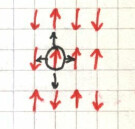
\includegraphics[scale=0.5]{images/1606337133.jpg}

Se utiliza como modelo para la condensación (es isomorfo con Ising)

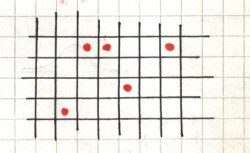
\includegraphics[scale=0.5]{images/1606337136.jpg}
 
\[
	Z_C = \sum_{\{ n_i \}}' \: \euler^{\beta e \sum_{\vm{ij}} n_i n_j }
	\qquad \qquad 
	\text{ con la restricción} \; \sum_i n_i = N
\] 
Paso al gran canónico porque $N$ está restringido y complica la sumatoria,
\[
	Z_{GC} = \sum_{N=0} \: z^N \: \sum_{\{ n_i \}}' \: \euler^{\beta e \sum_{\vm{ij}} n_i n_j }
\]
\[
	Z_{GC} = \sum_{\{ n_i \} = 0}^1 \: \euler^{ \beta \mu \sum_i n_i + \beta e \sum_{\vm{ij}} n_i n_j }
\]

Hago una analogia con los casos spin up y spin down respecto de sitio ocupado y sitio vacío,
respectivamente. Defino entonces
\[
	n_i = \frac{ S_i + 1 }{ 2 }
\]

Ahora podemos linkear la solución de lattice con el modelo de spin
\[
	\sum_i^N 1 = N  \qquad \qquad 
	\sum_{\vm{ij}} 1 = \gamma N \qquad \qquad 
	\sum_{\vm{ij}} S_i = \frac{\gamma}{2} \sum_{i=1}^N S_i
\]
y con esto deberíamos llegar a algo así como
\[
	Z_{GC} = \sum_{\{ S_i \} } \: \euler^{ (\beta \mu / 2 + \beta \gamma e / 4 ) 
	\sum_i^N S_i + \beta e/ 4 \sum_{\vm{i,j}} S_i S_j}
	\euler^{\beta N/2} \euler^{\beta e N/8} 
\]

Esto es la $Z_{GC}$ de Ising, porque en Ising tengo fijo $N$ (y no $N_+,N_-$) y en el lattice
el equivalente de $N$ es $N_+$ que sí fluctúa.

Podemos hacer la siguiente tablita 
\begin{center}
\begin{tabular}{l|l}
Ising & Lattice \\
\hline 
\# up & $N_{a+}$ \\
\# down & $N - N_{a+}$ \\
4J & $\vare $\\
$\euler^{2 \beta (\gamma J - m_0 H ) }$ & $z$ \\
$-\frac{A}{N} + \frac{1}{2} \gamma J - m_0 H$ &  $P $
\end{tabular}
\end{center}

 
\end{ejemplo}

\begin{ejemplo}{\bf Problema 2}

Consideraremos una solución exacta del problema de Ising.
Condiciones de contorno periódicas

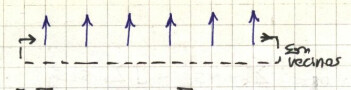
\includegraphics[scale=0.5]{images/1606337141.jpg}

En $H=0$ es $E=-JN$

\notamargen{Dibjo que no entendí bien de la carpeta en p47R: vínculos
desalineados (paredes de dominio).}

Con un cambio sutil (caso toy) de la combinación
up-up-up-down-up-up versus up-down-down-down-down-up que tienen $E=-JN+4J$
pero la magnetización es dferente porque son opuestos en signo.

La diferencia de energía con el inicial es
\[
	\frac{\Delta E}{N} = \frac{4J}{N} \to_{N\to \infty} 0
\]
el tamaño de la barrera de energía es $4J$ para cualquier $N$.
Se tiene $A=U-TS$ y $\vm{M}=0$
 
En $1D$ es $\vm{M}=0$ para cualquier $T>0$

\[
	E = - \mu H \sum S_i - J \sum_i S_i S_{i+1}
\]
\[
	Z_C = \sum_{\{ S_i \}} \euler^{ \beta H \sum_{i=1}^N S_i + J \sum^N_{i=1} S_i S_{i+1}}
\]
\[
	Z_{GC} = \sum_{S_1} \sum_{S_2} ... \sum_{S_N} \euler^{ \beta \mu H \sum_{i=1}^N (S_i+S_{i+1})/2 
	+ J \sum^N_{i=1} S_i S_{i+1}} =
	\sum_{S_1} \sum_{S_2} ... \sum_{S_N} \prod_{i=1}^N \euler^{ \beta \mu H (S_i+S_{i+1})/2 
	+ J S_i S_{i+1}}
\]
\[
	Z_{GC} =
	\sum_{S_1} \sum_{S_2} ... \sum_{S_N} 
	\euler^{ \beta \mu H (S_1+S_2)/2 + J S_1 S_2} - 
	\euler^{ \beta \mu H (S_2+S_3)/2 + J S_2 S_3}
\]
 
\[
	P = \begin{pmatrix}
	 \euler^{\beta(\mu H + J)} & \euler^{-\beta J} \\
	& \\ 
	 \euler^{-\beta J} &  \euler^{\beta(-\mu H + J)}
	\end{pmatrix}
\]
en la cual la primer fila es ``up'' y la segunda ``down''.
La cosa tiene una pinta del tipo
\[
	\sum_{S_1} \sum_{S_2} ... \sum_{S_N} S_N P_{S1 S2} P_{S2 S3} P_{S3 S4} ... P_N
\]
pero se tienen
\[
	\sum_{S_2} P_{S1 S2} P_{S2 S3} = (P^2)_{S_1,S_3} \qquad 
	\sum_{S_3} (P^2)_{S_1,S_3} P_{S3} P_{S4} = (P^3)_{S_1,S_4} 
\]
de manera que 
\[
	Z = \sum_{S_i} (P^N)_{S_i,S_i} = \text{Traza}(P^N)
\]
\[
	Z = \text{Tr}(P^N) = \lambda^N_+ + \lambda^N_- = 
	\lambda^N_+\left( 1 + \Frac{\lambda_-}{\lambda_+}^N \right) 
\]
\[
	Z \to \lambda^N_+ \qquad {N\to\infty}
\]

\[
	\lambda^N_+ = \euler^{\beta J N}
	\left[ \cosh(\beta \mu H) + \sqrt{ \sinh^2(\beta \mu H) + \euler^{-4\beta J} } \right]^N
\]
\[
	M \equiv \mu \vm{ \sum_{i=1}^N S_i } = \dpar{\log Z_N}{\beta H}
\]
\[
	M = \frac{ N \sinh(\beta \mu H) \beta \mu ( 1 + \cosh (\beta \mu H) ) }
	{  \cosh(\beta \mu H) + \sqrt{ \sinh^2(\beta \mu H) + \euler^{-4\beta J} } 
	\sqrt{ \sinh^2(\beta \mu H) + \euler^{-4\beta J} } }
\]
y entonces se tiene $M \to 0$ con $H \to 0$ no hay magnetización espontánea en Ising $1D$.

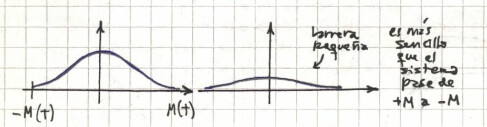
\includegraphics[scale=0.5]{images/1606337147.jpg}

\end{ejemplo}

\subsection{Ising en 2D}

\[
	E = - \mu H \sum S_i - J \sum_{\vm{i,j}} S_i S_j
\]

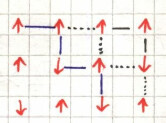
\includegraphics[scale=0.5]{images/1606337150.jpg}

Por más que no sean primeros vecinos, la correlación hace que la información llegue a lo largo de toda la red.
Esto va a dar lugar a los fenómenos críticos.

Usaremos la aproximación de Bragg-Williams (campo medio). Pensaremos en un sistema eqeuivalente
con una suma primada en primeros vecinos
\[
	E_i = - \mu H \sum S_i - J S_i \sum_{j}' S_j =
	- \mu S_i \left( H + \frac{J}{\mu} \sum_{j}' S_j \right) 
\]
y luego se reemplaza la suma sobre los vecinos por la suma de los $\gamma$ vecinos por el spin medio,
i.e. se hace $\sum' S_i \to \gamma \vm{S}$
\[
	E_i \approx -\mu S_i \left( H + \frac{J}{\mu} \gamma \vm{S} \right) 
\]

Esta aproximación pierde la información de correlaciones locales reemplazándola por correlaciones globales.
El $\vm{S} \sim 1$ (ver primer panel en la figura de abajo)

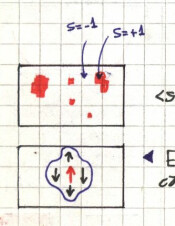
\includegraphics[scale=0.5]{images/1606337155.jpg}

El segundo panel de la figura es otra aproximación algo mejor; saco el spin y sus cuatro vecinos y hago
campo medio del resto. El $\vm{S}$ es el mismo para toda la red y eso debe valer con CPC o algo que tenga
sentido.

Sigamos con la aproximación más gruesa que es tomar uno solo y hacer campo medio con el resto
El paréntesis en la expresión de $E_i$ sería como un $H$ efectivo (local) y luego
\[
	Z_1 = \euler^{\beta\mu H_i } + \euler{-\beta\mu H_i } = 2 \cosh( \beta\mu H_i )
\]
\[
	Z_N = 2^N \cosh^N( \beta\mu H + \beta J \gamma \vm{S} )
\]
y entonces
\[
	\vm{S_i} = \frac{ \sum_{S_i=-1}^1 \: S_i \euler^{-\beta \mu H S_i } }{ 2 \cosh( \beta\mu H_i ) }
	= \tanh(\beta\mu H_i)
\]
y la ecuación de autoconsistencia
\[
	\vm{S_i} = \tanh( \beta\mu H + \beta J \gamma \vm{S} )
\]
que lleva a ? $\vm{s} = \tanh( \beta \mu H + \beta j \gamma \vm{s})$

Vemos grafiquito debajo de estas líneas

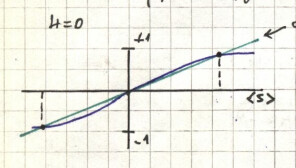
\includegraphics[scale=0.5]{images/1606337159.jpg}

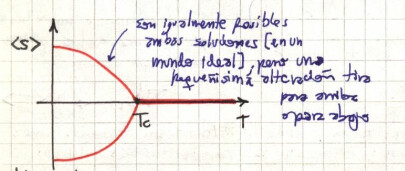
\includegraphics[scale=0.5]{images/1606337163.jpg}

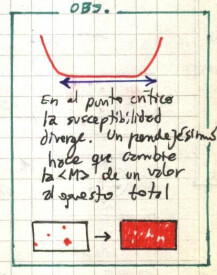
\includegraphics[scale=0.5]{images/1606337167.jpg}



\begin{ejemplo}{\bf Problema 4}
 
\end{ejemplo}

\begin{ejemplo}{\bf Problema 5 (planteo)}
 
\end{ejemplo}
% =================================================================================================
\section{Fenómenos críticos}
% =================================================================================================

Existe analogía entre sistemas magnéticos $(H,M)$ y gases $(p,V)$
\[
	H,M,T	\qquad \qquad \qquad p,V,T
\]
\[
	H \equiv P \qquad -M \equiv V
\]
\[
	dU = TdS + HdM + \mu dM 
\]
y con $N$ fijo,
\[
	T.dS = dU - H.dM	
\]
\[
	c_V = \dtot{Q}{T}|_V, \kappa_T = \dpar{V}{T}|_T
\]
\[
	A = U - TS \qquad dA = dT - TdS - SdT = HdM + \mu dM - SdT
\]

\[
	c_M = T\dtot{S}{T}|_M = T \dpar{S}{T}|_M = -T\dpar[2]{A}{T}|_M 
\]
\[
	\dpar{A}{T}|_{M,N} = -S \qquad \dpar[2]{A}{T}|_{M,N} = -\dpar{S}{T}|_{M,N}
\]
\[
	\chi_T \equiv \dpar{M}{H}|_T = \dpar{}{H}\left(\dpar{G}{H}|_T\right)_T = - \dpar[2]{G}{H}|_T
\]
\[
	G = U - TS -HM \qquad dG = dA - HdM - MdH = \mu dN - SdT - M dH
\]
\[
	M = \sum s_i = NL \qquad \chi_T = \dpar{NL}{H}|_T
\]
sabiendo que 
\[
	\overline{L} = \tanh ( \beta H \mu + \beta \gamma J \overline{L} )
\]
Derivando ambos lados:

dibujos

$L$ revienta en $T=T_c$

\notamargen{ \[
N \dpar{L}{H} = N \dpar{L}{T} \dpar{T}{H}
\] y la derivada parcial del medio revienta. }

y las derivadas segundas de $G$ discontinuas en $T_c$

Landau propone una teoría unificada de comportamiento de un sistema cerca del punto crítico.
Introduce el parámetro de orden $m_0$ que vale 0 si $T>T_c$ y $\neq 0$ si $T<T_c$.

La idea es expandir $ A = A(m_0) $.
Con $H=0$ el sistema es simétrico y entonces términos pares
\[
	t \equiv \frac{T-T_c}{T_c} = \frac{T}{T_c} -1  \qquad Y = \text{ Fuerza generalizada }
\]
\[
	\Psi( t, m_0,Y ) = \Psi_0( t, Y ) + r(t) m_0^2 + s(t) m_0^4
\]
\[	
	\dpar{\Psi}{m_0} = 0 \qquad  \qquad  \dpar[2]{\Psi}{m_0} \geq 0
\]
\[	
	\dpar{\Psi}{m_0} = 2 r(t) m_0 + 4 s(t) m_0^3 = 0 \qquad \qquad 
	\dpar{\Psi}{m_0} = 2 r(t) + 12 s(t) m_0^2 \geq 0
\]
\[	
	m_0^2 = -\frac{r(t)}{2s(t)}
\]
y con $m_0$ grande se tiene que $s(t)>0$ controla la concavidad.

Elegimos
\[
	r > 0 \quad T > T_c \quad \rightarrow \quad \text{ mínimo en } m_0 = 0
\]
\[
	r < 0 \quad T < T_c \quad \rightarrow \quad \text{ mínimos en } m_0 \neq 0
\]
siendo estos mínimos localizados en $\pm \sqrt{ -r(t)/(2s(t))}$.
\[
	\Psi \text{ continua en } t=0 \rightarrow r=0 \text{ en } T=T_c
\]
\[
	r(t) = \alpha_2 t \qquad \qquad s(t) = 2 \alpha_4 > 0 \quad \text{ así }
\]
\[
	2 \alpha_2 t - 3 \alpha_2 t = - \alpha_2 t = -\alpha_2 \left( \frac{T}{T_c} - 1 \right)\geq 0
\]
y esta cuenta significa que si $T<T_c$ es $\alpha_2 <0$ y si $T>T_c$ es $\alpha_2 >0$

dibujo

\[
	\Psi = \Psi_0 - \frac{\alpha_2^2t^2}{4\alpha_4} \qquad T < T_c
\]
\[
	\Psi = \Psi_0 \qquad T>T_c
\]
\[
	C_M = - T \dpar[2]{A}{T}|_M = \begin{cases}
	                        \displaystyle -T \dpar[2]{\Psi_0}{T} \\
	                        \\
	                        \displaystyle -T \dpar[2]{\Psi_0}{T} + 2 T \frac{\alpha_2}{4\alpha_4} \frac{1}{T_c^2}
	                        \end{cases}
\]

Si hay campo externo :
\[
	\Psi = \Psi_0 + \alpha_2 t m_0^2 + 2 \alpha_4 m_0^4 - f m_0
\]
\[
	\dpar{\Psi}{m_0} = 2 \alpha_2 t m_0 + 8 \alpha_4 m_0^3 - f =  0
\]
y derivando contra $f$,
\[
	2 \alpha_2 t \dtot{m_0}{f} + 24 \alpha_4 m_0^2 \dtot{m_0}{f} - 1 = 0
\]
\[
	\chi = \dtot{m_0}{f} = \frac{1}{2\alpha_2 t + 24 \alpha_4 m_0^2}
\]

Con $f \to 0$ recordamos
\[
	T > T_c \quad m_0 = 0 \quad \rightarrow \quad \chi \to \frac{1}{2\alpha_2 t} = 
	\frac{T_c}{2\alpha_2(T-T_c)}
\]
\[
	T < T_c \quad m_0 = -\frac{\alpha_2 t}{4\alpha_4} \quad \rightarrow \quad \chi \to 
	-\frac{1}{4\alpha_2 t} = -\frac{T_c}{4\alpha_2(T-T_c)}
\]

Ambos revienta en $T_c$

DIBUJO

% =================================================================================================
\section{Exponentes críticos}
% =================================================================================================

\begin{itemize}
 \item Al cruzar el punto crítico el parámetro de orden crece.
 \item En la vecindad del punto crítico el sistema sobrelleva procesos de ajuste, entonces
 hay grandes fluctuaciones.
 \item Algunas fluctuaciones termodinámicas tienen diferentes comportamientos.
\end{itemize}

Los exponentes críticos describen la naturaleza de las singularidades en el punto crítico.
Son seis: $ \alpha, \beta, \gamma, \delta, \eta, \nu $
\[
	t = \frac{T-T_c}{T_c} \qquad \text{ parámetro } 
\]

Cerca del punto crítico las funciones termodinámicas pueden escribirse como:
\[
	f(t) = A t^\lambda ( 1 + Bt^y + ... ), \quad y > 0 
\]
y tenemos un exponente crítico $\lambda$
\[
	\lambda = \lim_{t\to 0} \frac{\log f(t)}{\log t}  \begin{cases}
	                                                   < 0 \quad \text{ diverge }  f(t) \\
	                                                   > 0 \quad \text{ a 0 } \\
	                                                   = 0 \quad \text{ divergencia logarítmica } 
	                                                  \end{cases}
\]

\begin{center}
\begin{tabular}{lll}
 & expresión & rango \\
\hline
$C_M, C_v$ & $(-t)^{-\alpha}$ & $t < 0$  \\
 & $ (t)^{-\alpha}$ & $t > 0$\\
$M$  & $ (-t)^\beta $ & $t < 0 $ \\
$\dpar{V}{p} \propto \kappa_T, \chi_T $ & $ (-t)^{-\gamma '}$  & $t < 0$ \\
 & $ (t)^{-\gamma'} $ & $t > 0$ \\
$H$ & $ |M|^\delta $ & $t=0$ \\
$P$ & $ \rho^\delta $ & $t=0$ 
\end{tabular}
\end{center}

\notamargen{Justamente $M$ es el parámetro de orden y $M=0$ con $t>0$} 

Se cumplen ciertas desigualdades entre exponentes:
\[
	\text{ Rushbroke } \qquad \qquad 2 \leq \gamma ' + 2 \beta + \alpha ' \quad (H=0)  
\]
\[
	\text{ Griffiths } \qquad \qquad \alpha ' + \beta(1+\delta) \geq 2  
\]

\subsection{Exponentes críticos Van Der Waals} 

\[
	\left( p + \frac{an^2}{V^2}\right) (V-nb)= nRT
\]
\[
	\overline{p} = \frac{p}{p_c} \quad \to \quad \frac{p-p_c}{p_c} = \overline{p}-1 = \mathcal{p}, v, t
\]
Y como en $T=T_c$ es $ t = 0 $ entonces 
\[
	2p(1+\frac{7v}{2} + 4v^2 + \frac{3v^2}{2}) = -3v^3 + 8t(1+2v + v^2)
\]
pero $t=0$,
\[
	p = -\frac{3}{2} v^3 \left(1+\frac{7v}{2} + 4v^2 + \frac{3v^2}{2}\right)^{-1}
\]
\[
	\delta = 3
\]

Para la teoría de Landau es:
\[
	M = m_0 = \Frac{\alpha_2}{2\alpha_4}^{1/2}(T_c-T)^{1/2} \quad \to \quad \beta = 2
\]
\[
	\chi = \begin{cases}
		\propto \frac{1}{t} \quad t>0 \\
		\propto \frac{1}{-t} \quad t<0 \\
	       \end{cases} 
	\quad \to \quad \gamma = \gamma ' = 1       
\]
$C_H$ tiene $\alpha \approx 0$, $\alpha ' \approx 0 $ (ver que no dependen de $t$ )

\notamargen{Las transformaciones de primer orden $\dpar{G}{T}, \dpar{G}{x}$ son discontinuas.}

\subsection{Sobre trabajo y relación $p,V$ [mover]}

\[ 
	dU = dQ - p dV
\]

DIBUJO 

El sistema entrega trabajo al entorno si $ pdV > 0 $ y entonces $ dV > 0 $ (expansión)
pues $ p > p_{ext} $

El sistema absorbe energía en forma de trabajo si $ pdV < 0 $ y entonces $ dV < 0 $ (compresión)
pues $ p < p_{ext} $
\notamargen{$p$ y $V$ no varían separadamente; si $p$ sube entonces $V$ baja.}

\[
	\text{ Si } p > p_{ext} \to \text{ exp. } dV > 0 (dp < 0)
\]
\[
	\text{ Si } p < p_{ext} \to \text{ comp. } dV < 0 (dp > 0)
\]
y $V$ drecrece con $p$ subiendo.

\[
	\underbrace{p}_{\text{intensiva}} \underbrace{dV}_{\text{extensiva}} = 
	dW \qquad \qquad p>0 \text{ siempre }
\]

Para el sistema magnético si $ H > 0 $ entonces $ dM > 0 $
\[
	dU = dQ + H dM
\]
donde el segundo miembro es el trabajo magnético realizado por el sistema.

Si el sistema se ordena $dM>0$ y baja su energía y por ende hace trabajo.
\notamargen{Este sistema hace trabajo no mecánico.}

\subsection{Comentarios varios [mover]}

Los efectos de la estadística cuántica surgen de la indistinguibilidad de las partículas.
\[
	\frac{\lambda^3}{v} \ll 1 \text{(Clásico)}
\]
\[
	\frac{\lambda^3}{v} \approx 1 \text{(Cuántico)}
\]
Cuando $\lambda^3/v \approx 1$ surgen efectos cuánticos y tiene importancia la estadística de las
partículas (BE o FD).

Para un sistema de cuasipartículas es $\mu=0$. En general,
\[
	\mu = \mu(T)
\]
es un valor único para el sistema y depende de la temperatura.
\begin{itemize}
 \item gas ideal
 \subitem clásico : partículas no interactuantes. $T$ alta y $v$ alto.
 \subitem cuántico : partículas no interactuantes. $T$ baja y $v$ bajo.
 \item bosones 
 \subitem partículas
 \subitem cuasipartículas : no tienen masa. $N$ no está fijo.
 \item fermiones 
 \subitem partículas
\end{itemize}


\subsection{Para apéndice [mover]}

\[
	\Gamma \left( m +\frac{1}{2} \right) = \left( m -\frac{1}{2} \right) \left( m -\frac{3}{2} \right)
	... \frac{3}{2} \cdot \frac{1}{2} \cdot \Gamma(1/2), m \in \mathbb{N}
\]
\[
	\Gamma(3/2) = \Gamma(1+ 1/2) =\frac{1}{2} \Gamma(1/2) = \frac{\pi^{1/2}}{2}
\]

Calculando momentos permitidos en una caja es de lo más divertido y resulta 
\[
	\frac{V}{h^3} d|\vb{p}| = 1 
\]
donde $ d\vb{p} = dx \hat{x} + dy \hat{y}+ dz \hat{z}$ y $ d|\vb{p}| = dx dy dz $   en cartesianas.
En cambio en esféricas es
\[
	4 \pi p^2 \frac{V}{h^3} dp = 1
\]
\[
	1 = \frac{ V \hbar dk \hbar^2 k^2 4 \pi  }{ h^3 } = \frac{V 4\pi k^2 dk}{ (2\pi)^3 }
\]

Para pasaje de $\sum_{\vb{p}}$ a $\int d^3p d^3q $ utilizamos los siguientes 
\[
	dp_x dx  = h \qquad \text{ Incertidumbre }
\]
y entonces 
\[
	d^3p d^3x = h^3 \quad \to \quad \frac{1}{h^3 }d^3p d^3x = 1 
\]
y parece que 
\[
	\frac{V}{h^3} \int d^3 p = 1 
\]
\notamargen{Anoté que no estoy seguro de esta última cuenta, en lápiz tenue.}

\subsection{Fenómenos críticos (1)}

Por $ T > T_C $ el sistema  es dominado por la entropía $S$; se comporta normalmente. Con $ T < T_C $
hay algo que rompe la simetría y hay una dirección preferencial.
\[
	\frac{ N_{++} }{ N y/2 } = \Frac{ N_{+} }{ N }^2
\]
La aproximación de campo medio es esto de arriba y se tiene $ 1/ V \log Q^{BG}$ donde quiero buscar el $A$.
El término más grande será $\bar{L}$ y será el que maximiza la sumatoria

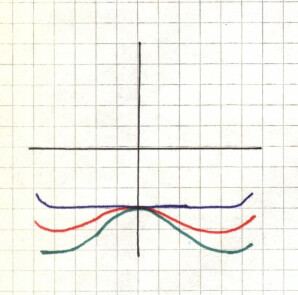
\includegraphics[scale=0.4]{images/1606337033.jpg}

Aquí el sistema se parece a un fluido

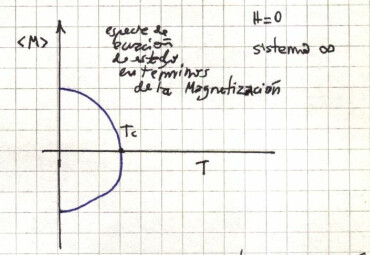
\includegraphics[scale=0.4]{images/1606337037.jpg}

Para $T<T_C$ es como una transición de fase de primer orden. El $C_V$ diverge en $T_C$ con sistema infinito,
y el $C_V$ es máximo en $T_C$ con sistema finito.
Los exponentes críticos: buceamos analogía entre fluidos y magnetización.
Luego del $P_C$ surgen modos colectivos de agrupamiento (sistema de spines) y comparo $H,M,T \to P,V,T$

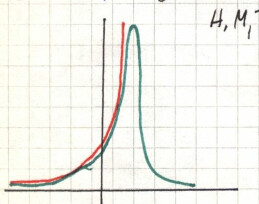
\includegraphics[scale=0.4]{images/1606337041.jpg}

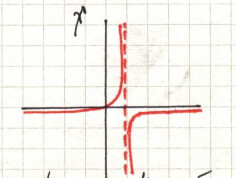
\includegraphics[scale=0.4]{images/1606337044.jpg}

Por debajo del $T_C$ hay dominios de magnetización; dirección preferencial de los spines.
Se habla de un {\it parámetro de orden}.

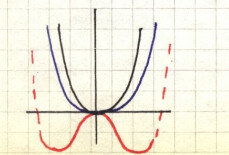
\includegraphics[scale=0.4]{images/1606337048.jpg}

Landau propone una explicación de lo que pasa en el punto crítico.

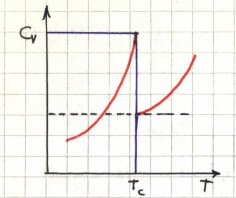
\includegraphics[scale=0.4]{images/1606337054.jpg}

Recuerda el resultado de Bragg-Williams (campo medio). Me da una visión de grano grueso.
Pero borra las correlaciones.

Las correlaciones en $T_C$ rompen la simetría que teníamos (sistema conducido por la entropía $S$)

Los fluidos tienen un $P_C$ pero no se rompe ninguna simetría; esto es apropiado para sistemas que
pueden manifestar una simetría en el espacio.

Landau nos ubica cerca del $P_e$ entonces lo relevante es el parámetro de orden $m_0$: desarrollo del potencial
termodinámico en términos de $m_0$ y de ahí me quedo con potencias pares para que no dependa del signo de los
spines.

Con un campo externo se rompe la simetría del problema. Se corre el punto de transición desde cero.
$\chi \to \infty$ en $T=T_C$

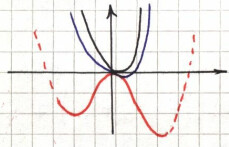
\includegraphics[scale=0.4]{images/1606337058.jpg}

Los exponentes críticos intentan caracterizar cómo varían ciertas cantidades en las proximidades de dicho punto.


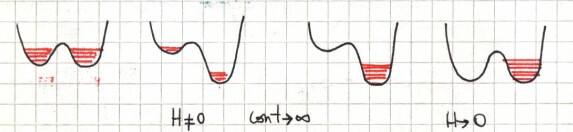
\includegraphics[scale=0.4]{images/1606337061.jpg}

Habría que definir cuántos exponentes críticos son necesarios para describir un sistema cerca del punto crítico.

\subsection{Fenómenos críticos (2)}

Se quiere caracterizar a los sistemas con exponentes críticos; pero con un $H$ reducido.

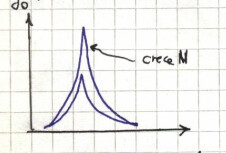
\includegraphics[scale=0.4]{images/1606337120.jpg}

Van der Waals es una ecuación en términos de campo medio; la expresamos en distancias relaticas a los puntos
críticos.

Comparando con valores reales vemos que Van der Waals y Landau no dan parecido: y es así porque son teorías de
campo medio.
En la vecindad del punto crítico se desarrolla en términos del parámetro de orden. Consideramos exponentes
yendo en las dos direcciones.

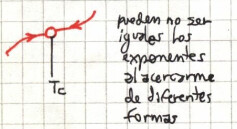
\includegraphics[scale=0.4]{images/1606337124.jpg}

Si un potencial termodinámico es una función homogénea generalizada entonces todos los potenciales 
termodinámicos lo son.
Los exponentes críticos pueden relacionarse con $p,q$ y entonces con dos números tengo toda la información
del sistema.

Las distancias de correlación empiezan a crecer en $T_C$.

Como $\xi$ diverge en un $\sim T_C$ entonces la distancia de correlación es mucho mayor al tamaño de las
celdas; éstas están muy correlacionadas. Se da que $LL$ es mucho menor a la distancia de correlación.

Podemos hacer un proceso de ``renormalización''; reemplazar una celdad por un spin efectivo $+$ o $-$
para toda la celda.

Como estamos cerca de $T_C$ y tenemos grandes dominios no tendremos tableros de ajedrez.
Cerca del punto crḉitico ambos sistemas serían prácticamente indistinguibles (hipótesis de Kadanoff).

En el punto crítico la distancia de correlación se va a infinito. A consecuencia de esta transformación
podemos porbar que la energía libre de Gibbs es una función homogénea generalizada.
El hamiltoniano cambia de acuerdo a un escaleo en las variables análogo al que se hizo para la 
transformación.
Las dependencias aparecen en los parámetros del hamiltoniano.
La red se hace autosimilar (igual a sí misma) pero escaleada.

\begin{ejemplo}{Problema 2}
Tenemos
\[
	\beta P = \sum_{n> 1}^\infty \: B_n p^n
\]
y solicitan desarrollos del virial para $E,S$, se ve que es conveniente usar $A=U-TS$ de modo que
$dA = -p dV - S dT$ y 
\[
	A = A^\text{gas ideal} + A^\text{exceso}
\]
de modo que
\[
	P = P^\text{GI} + P^\text{e} \qquad \quad S = S^\text{GI} + S ^\text{e}
\]

Los problemas 3,4 salen con los resultados del problema 2.
\end{ejemplo}

El punto crítico es un punto fijo de la transformación

\begin{itemize}
 \item $\lambda_i > 1 $ indican la direccióin de crecimiento
 \item $\lambda_i = 1 $ irrelevantes.
 \item $\lambda_i < 1 $ indiferentes; se van a cero y no aportan.
\end{itemize}

Criterio de la mayoría: tomo el signo. Mapeo una red triangular en una red traingular; tres spines
son un super spin. $V$ es el término de superficie.

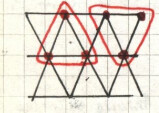
\includegraphics[scale=0.6]{images/1606337128.jpg}

Con los exponentes críticos hicimos una hipótesis de ``scaling''; entonces con un par de exponentes
críticos podríamos resolver el problema habiendo definido unas funciones homogéneas.
Kadanoff dice o lleva a que los problemas son autosimilares. Wilson dice o lleva a que la función
de partición se conserva y queda libre el $H$.




% \bibliographystyle{CBFT-apa-good}	% (uses file "apa-good.bst")
% \bibliography{CBFT.Referencias} % La base de datos bibliográfica

\end{document}

